% ============================================================
%  CS3401 – Chapter 1: Introduction to Algorithm Design
% ============================================================
\documentclass[aspectratio=169]{beamer}
% ============================================================
%  CS3401 – Algorithm Design and Analysis
%  Shared Beamer Theme (input this file in every chapter)
%  Prince Sattam Bin Abdulaziz University – CCES
% ============================================================

% ---------- PACKAGES ----------------------------------------
\usepackage[utf8]{inputenc}
\usepackage[T1]{fontenc}
\usepackage{lmodern}
\usepackage{amsmath,amssymb,amsthm}
\usepackage{tikz}
\usepackage{pgfplots}
\usepackage{booktabs}
\usepackage{xcolor}
\usepackage{graphicx}
\usepackage{listings}
\usepackage[normalem]{ulem}
\usepackage{algorithm}
\usepackage{algpseudocode}
\usepackage{multicol}
\usepackage{array}
\usepackage{colortbl}
\usepackage{tabularx}
\usepackage{makecell}

\usetikzlibrary{
  arrows.meta, shapes.geometric, shapes.symbols,
  positioning, calc, fit, backgrounds,
  decorations.pathreplacing, decorations.markings,
  matrix, chains, trees
}
\pgfplotsset{compat=1.18}

% ---------- COLOR PALETTE -----------------------------------
\definecolor{PrimaryDark}{RGB}{10,72,92}
\definecolor{PrimaryMid}{RGB}{18,114,145}
\definecolor{PrimaryLight}{RGB}{185,224,238}
\definecolor{AccentOrange}{RGB}{210,103,22}
\definecolor{AccentYellow}{RGB}{252,198,40}
\definecolor{SuccessGreen}{RGB}{32,122,66}
\definecolor{AlertRed}{RGB}{172,46,46}
\definecolor{CodeBg}{RGB}{244,246,250}
\definecolor{DarkText}{RGB}{28,32,40}
\definecolor{LightRule}{RGB}{210,225,232}
\tikzset{processstep/.style={draw=PrimaryMid, fill=PrimaryLight!35, rounded corners=2pt,
  align=center, minimum width=4.2cm, minimum height=0.55cm, font=\small}}

% ---------- BEAMER SETTINGS ---------------------------------
\setbeamertemplate{navigation symbols}{}
\setbeamertemplate{caption}[numbered]

% Fonts
\setbeamerfont{normal text}{size=\small}
\setbeamerfont{title}{series=\bfseries,size=\LARGE}
\setbeamerfont{subtitle}{series=\normalfont,size=\large}
\setbeamerfont{frametitle}{series=\bfseries,size=\large}
\setbeamerfont{framesubtitle}{series=\normalfont,size=\small}
\setbeamerfont{block title}{series=\bfseries,size=\normalsize}
\setbeamerfont{footline}{size=\tiny}
\addtobeamertemplate{frame begin}{\small\enlargethispage{1cm}}{}
\setlength{\tabcolsep}{2pt}

% Colors
\setbeamercolor{normal text}{fg=DarkText,bg=white}
\setbeamercolor{frametitle}{bg=PrimaryDark,fg=white}
\setbeamercolor{title}{fg=white}
\setbeamercolor{subtitle}{fg=PrimaryLight}
\setbeamercolor{author}{fg=white}
\setbeamercolor{date}{fg=PrimaryLight}
\setbeamercolor{institute}{fg=PrimaryLight}
\setbeamercolor{block title}{bg=PrimaryMid,fg=white}
\setbeamercolor{block body}{bg=PrimaryLight!35,fg=DarkText}
\setbeamercolor{block title alerted}{bg=AlertRed,fg=white}
\setbeamercolor{block body alerted}{bg=AlertRed!12,fg=DarkText}
\setbeamercolor{block title example}{bg=SuccessGreen,fg=white}
\setbeamercolor{block body example}{bg=SuccessGreen!12,fg=DarkText}
\setbeamercolor{itemize item}{fg=PrimaryMid}
\setbeamercolor{itemize subitem}{fg=AccentOrange}
\setbeamercolor{enumerate item}{fg=PrimaryMid}
\setbeamercolor{enumerate subitem}{fg=AccentOrange}
\setbeamercolor{alerted text}{fg=AlertRed}
\setbeamercolor{structure}{fg=PrimaryMid}
\setbeamercolor{section in toc}{fg=PrimaryDark}
\setbeamercolor{section in toc shaded}{fg=PrimaryDark}
% override Beamer's transparency-based shading so TOC entries stay fully visible
\setbeamertemplate{section in toc shaded}{\inserttocsection\par}
\setbeamercolor{subsection in toc}{fg=PrimaryMid}
\setbeamercolor{footer rule}{bg=LightRule}

% Item symbols
\setbeamertemplate{itemize item}{%
  \scriptsize\raise1.5pt\hbox{\color{PrimaryMid}$\blacktriangleright$}}
\setbeamertemplate{itemize subitem}{%
  \scriptsize\raise1pt\hbox{\color{AccentOrange}$\bullet$}}
\setbeamertemplate{itemize subsubitem}{%
  \scriptsize\raise1pt\hbox{\color{PrimaryDark}$\circ$}}
\setbeamertemplate{enumerate item}{%
  \color{PrimaryMid}\textbf{\insertenumlabel.}}

% Frame title
\makeatletter
\setbeamertemplate{frametitle}{%
  \nointerlineskip
  \begin{beamercolorbox}[wd=\paperwidth,ht=2.4em,dp=0.9em,%
                         leftskip=1.2em,rightskip=1.2em]{frametitle}
    \usebeamerfont{frametitle}\insertframetitle\strut
    \ifx\insertframesubtitle\@empty\else
      \hspace{0.6em}\textcolor{PrimaryLight!80}{\footnotesize|}\hspace{0.4em}%
      {\usebeamerfont{framesubtitle}\textcolor{PrimaryLight}\insertframesubtitle}%
    \fi
  \end{beamercolorbox}
  \nointerlineskip
  \begin{beamercolorbox}[wd=\paperwidth,ht=0.3pt,dp=0pt]{structure}
  \end{beamercolorbox}
}
\makeatother

% Footer
\setbeamertemplate{footline}{%
  \begin{beamercolorbox}[wd=\paperwidth,ht=0.4pt,dp=0pt]{footer rule}{}
  \end{beamercolorbox}
  \leavevmode
  \hbox{%
    \begin{beamercolorbox}[wd=0.60\paperwidth,ht=1.8em,dp=0.6em,leftskip=1em]{normal text}%
      \textcolor{PrimaryDark}{\tiny\textbf{CS3401} \textendash{} Algorithm Design \& Analysis%
        \quad\textbar\quad CCES, PSAU}%
    \end{beamercolorbox}%
    \begin{beamercolorbox}[wd=0.40\paperwidth,ht=1.8em,dp=0.6em,rightskip=1em,right]{normal text}%
      \textcolor{PrimaryDark}{\tiny\insertshorttitle%
        \quad\textbar\quad\insertframenumber\,/\,\inserttotalframenumber}%
    \end{beamercolorbox}%
  }%
}

% Title page
\setbeamertemplate{title page}{%
  
\begin{tikzpicture}[remember picture,overlay]
    \fill[PrimaryDark](current page.north west) rectangle (current page.south east);
    \fill[PrimaryMid,opacity=0.45]
      ([shift={(2.5cm,-2.5cm)}]current page.north east) circle(5.5cm);
    \fill[AccentOrange,opacity=0.10]
      ([shift={(-1.5cm,2.0cm)}]current page.south west) circle(4.2cm);
    \draw[white,opacity=0.08,line width=40pt]
      ([shift={(0cm,-0.5cm)}]current page.north west)
      to[out=-30,in=210]
      ([shift={(0cm,0.5cm)}]current page.south east);
  \end{tikzpicture}%
  \vspace{0.7cm}
  \begin{center}
    {\tiny\textcolor{PrimaryLight}{\textbf{CCES} \textendash{}
      College of Computer Engineering and Sciences}}\\[0.2em]
    {\tiny\textcolor{PrimaryLight}{Prince Sattam Bin Abdulaziz University}}\\[1.2em]
    {\footnotesize\textcolor{AccentYellow}{\textbf{CS3401 \textendash{} Algorithm Design and Analysis}}}\\[1.5em]
    \textcolor{PrimaryMid}{\rule{0.55\textwidth}{0.6pt}}\\[0.9em]
    {\Large\usebeamerfont{title}\textcolor{white}{\inserttitle}}\\[0.4em]
    {\small\usebeamerfont{subtitle}\textcolor{PrimaryLight}{\insertsubtitle}}\\[0.7em]
    \textcolor{PrimaryMid}{\rule{0.55\textwidth}{0.6pt}}\\[1.2em]
    {\footnotesize\textcolor{PrimaryLight}{\insertdate}}\\[0.6em]
    % Instructors row
    \begin{tikzpicture}[baseline=(current bounding box.center)]
      % Dr. Khalil – rounded photo
      \begin{scope}
        \clip (-3.2,0) circle (0.58cm);
        \node at (-3.2,0)
          {
\includegraphics[width=1.16cm,height=1.16cm,keepaspectratio=false]{khalil}};
      \end{scope}
      \draw[white,line width=0.9pt] (-3.2,0) circle (0.58cm);
      \node[text=white,font=\scriptsize\bfseries,anchor=west] at (-2.54,0)
        {Dr.\ Khalil Chebil};
      % Dr. Esraa – placeholder circle
      \draw[white,line width=0.9pt] (1.2,0) circle (0.58cm);
      \node[text=PrimaryLight,font=\normalsize\bfseries] at (1.2,0) {E};
      \node[text=white,font=\scriptsize\bfseries,anchor=west] at (1.86,0)
        {Dr.\ Esraa};
    \end{tikzpicture}
  \end{center}%
}

% Auto section-divider slide — background set via Beamer color system for reliability
\AtBeginSection[]{%
  {%
    \setbeamercolor{background canvas}{bg=PrimaryDark}%
    \begin{frame}[plain,noframenumbering]
      \begin{tikzpicture}[remember picture,overlay]
        \fill[PrimaryMid,opacity=0.35]
          ([shift={(0cm,-1.5cm)}]current page.north) circle(6.5cm);
        \node[text=white,opacity=0.06,font=\fontsize{120}{120}\bfseries]
          at ([shift={(-1cm,0cm)}]current page.center)
          {\insertsectionnumber};
      \end{tikzpicture}
      \vfill
      \begin{center}
        {\large\textcolor{AccentYellow}{\textbf{Section \insertsectionnumber}}}\\[0.6em]
        {\LARGE\textcolor{white}{\textbf{\insertsectionhead}}}
      \end{center}
      \vfill
    \end{frame}
  }%
}

% ---------- LISTINGS STYLE ----------------------------------
\lstset{
  basicstyle=\ttfamily\footnotesize,
  backgroundcolor=\color{CodeBg},
  keywordstyle=\color{PrimaryMid}\bfseries,
  commentstyle=\color{SuccessGreen}\itshape,
  stringstyle=\color{AccentOrange},
  numberstyle=\tiny\color{gray!70},
  frame=tb,
  framerule=0.5pt,
  rulecolor=\color{PrimaryLight},
  numbers=left,
  numbersep=6pt,
  showstringspaces=false,
  breaklines=true,
  tabsize=2,
  xleftmargin=1.8em,
  framexleftmargin=1.8em,
  captionpos=b,
  language=Java,
  morekeywords={var,let,const}
}

% ---------- PSEUDOCODE STYLE --------------------------------
\algrenewcommand\algorithmicprocedure{\textbf{Algorithm}}
\algrenewcommand\algorithmicfunction{\textbf{Function}}
\algrenewcommand\algorithmicif{\textbf{if}}
\algrenewcommand\algorithmicelse{\textbf{else}}
\algrenewcommand\algorithmicthen{\textbf{then}}
\algrenewcommand\algorithmicwhile{\textbf{while}}
\algrenewcommand\algorithmicfor{\textbf{for}}
\algrenewcommand\algorithmicforall{\textbf{for all}}
\algrenewcommand\algorithmicreturn{\textbf{return}}
\algrenewcommand\algorithmicend{\textbf{end}}
\algrenewcommand\algorithmicdo{}
\algrenewcommand\algorithmicrequire{\textbf{Input:}}
\algrenewcommand\algorithmicensure{\textbf{Output:}}

% ---------- CUSTOM COMMANDS ---------------------------------
\newcommand{\bigO}[1]{$\mathcal{O}(#1)$}
\newcommand{\bigTheta}[1]{$\Theta(#1)$}
\newcommand{\bigOmega}[1]{$\Omega(#1)$}
\newcommand{\highlight}[1]{\colorbox{AccentYellow!55}{\strut #1}}
\newcommand{\important}[1]{\textcolor{AlertRed}{\bfseries #1}}
\newcommand{\keyword}[1]{\textcolor{PrimaryMid}{\bfseries #1}}
\newcommand{\concept}[1]{\textcolor{AccentOrange}{\bfseries #1}}

% Colored table column types
\newcolumntype{H}{>{\columncolor{PrimaryDark}\color{white}\bfseries\centering\arraybackslash}m{2.5cm}}
\newcolumntype{Z}{>{\columncolor{PrimaryLight!40}\centering\arraybackslash}m{2cm}}

% Reference boxes
\newcommand{\refbox}[1]{%
  \begin{beamercolorbox}[rounded=true,shadow=false,leftskip=0.5em,rightskip=0.5em,%
                          ht=1.6em,dp=0.5em]{block title}
    \small\textit{Reference:} #1
  \end{beamercolorbox}%
}

% Inline complexity tag
\newcommand{\ctag}[1]{%
  \hfill\tikz[baseline]{\node[fill=AlertRed,text=white,rounded corners=2pt,
    font=\bfseries\scriptsize,inner sep=2pt,outer sep=0pt]{$\mathcal{O}(#1)$};}%
}


\title[Ch.\,1 -- Introduction]{Chapter 1}
\subtitle{Introduction to Algorithm Design}
\date{Academic Year 2026\,--\,2027}

% ── References ──────────────────────────────────────────────
% Levitin, "Introduction to the Design and Analysis of Algorithms", 3rd ed.
% Skiena, "The Algorithm Design Manual", 2nd ed.
% Cormen et al., "Introduction to Algorithms", 3rd ed.
% ─────────────────────────────────────────────────────────────

\begin{document}

\begin{frame}[plain]
  \titlepage
\end{frame}

% ── Outline ─────────────────────────────────────────────────
\begin{frame}{Chapter Overview}
  \begin{center}
    \begin{minipage}{0.85\textwidth}
      \tableofcontents[hideallsubsections,sectionstyle=show/shaded]
    \end{minipage}
  \end{center}
\end{frame}

% ============================================================
\section{Why Algorithms Matter}
% ============================================================

\begin{frame}{The Invisible Engine Behind Modern Technology}
  \begin{columns}[T]
    \column{0.55\textwidth}
      Every second:
      \begin{itemize}
        \item \textbf{Google} processes $>$100\,000 search queries
        \item \textbf{Spotify} streams to $>$600 million users
        \item \textbf{GPS} recalculates routes for millions of drivers
        \item \textbf{Banks} clear thousands of transactions
      \end{itemize}
      \vspace{0.5em}
      \begin{alertblock}{The Question}
        What tells a computer \emph{how} to solve these problems
        correctly and at speed?
      \end{alertblock}
    \column{0.40\textwidth}
      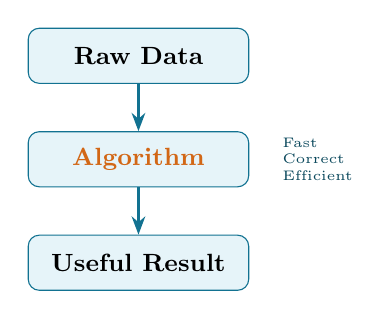
\begin{tikzpicture}[
        node/.style={draw=PrimaryMid,fill=PrimaryLight!35,rounded corners=4pt,
                     font=\small\bfseries,inner sep=5pt,minimum width=2.8cm,
                     minimum height=0.7cm,text centered},
        arr/.style={-{Stealth},PrimaryMid,thick}
      ]
        \node[node] (data) {Raw Data};
        \node[node,below=0.6cm of data] (algo) {\textcolor{AccentOrange}{Algorithm}};
        \node[node,below=0.6cm of algo] (result) {Useful Result};
        \draw[arr] (data)--(algo);
        \draw[arr] (algo)--(result);
        \node[right=0.3cm of algo,font=\tiny,text=PrimaryDark,align=left]
          {Fast\\Correct\\Efficient};
      \end{tikzpicture}
  \end{columns}
\end{frame}

\begin{frame}{A Motivating Example: Route Planning}
  \begin{columns}[T]
    \column{0.50\textwidth}
      \textbf{Problem:} Given a map with $n$ locations and road distances,
      find the \emph{shortest path} from A to B.
      \vspace{0.5em}
      \begin{itemize}
        \item With 10 cities there are $\approx 181\,000$ possible routes
        \item With 20 cities: $\approx 6\times10^{16}$ routes
        \item Checking them all is \important{impossible}
      \end{itemize}
      \vspace{0.5em}
      \begin{exampleblock}{Algorithm to the Rescue}
        Dijkstra's algorithm finds the shortest path among millions of
        nodes in \emph{milliseconds}.
      \end{exampleblock}
    \column{0.45\textwidth}
      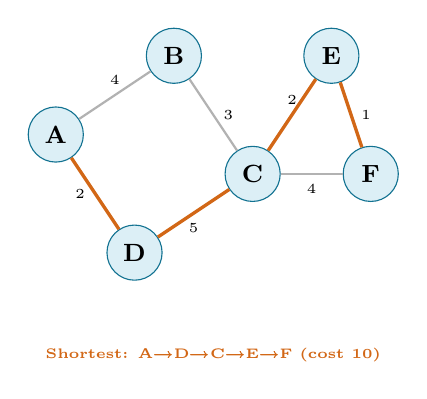
\begin{tikzpicture}[
        city/.style={circle,draw=PrimaryMid,fill=PrimaryLight!50,
                     font=\bfseries\small,minimum size=0.7cm},
        road/.style={draw=gray!60,thick},
        best/.style={draw=AccentOrange,very thick}
      ]
        \node[city] (A) at (0,2.5) {A};
        \node[city] (B) at (1.5,3.5) {B};
        \node[city] (C) at (2.5,2.0) {C};
        \node[city] (D) at (1.0,1.0) {D};
        \node[city] (E) at (3.5,3.5) {E};
        \node[city] (F) at (4.0,2.0) {F};
        \draw[road] (A)--(B) node[midway,above,font=\tiny]{4};
        \draw[road] (A)--(D) node[midway,left,font=\tiny]{2};
        \draw[road] (B)--(C) node[midway,right,font=\tiny]{3};
        \draw[road] (D)--(C) node[midway,below,font=\tiny]{5};
        \draw[road] (C)--(E) node[midway,above,font=\tiny]{2};
        \draw[road] (E)--(F) node[midway,right,font=\tiny]{1};
        \draw[road] (C)--(F) node[midway,below,font=\tiny]{4};
        % Highlight shortest path A->D->C->E->F
        \draw[best] (A)--(D)--(C)--(E)--(F);
        \node[font=\tiny\bfseries,text=AccentOrange] at (2,-0.3)
          {Shortest: A→D→C→E→F (cost 10)};
      \end{tikzpicture}
  \end{columns}
\end{frame}

% ============================================================
\section{What is an Algorithm?}
% ============================================================

\begin{frame}[shrink=12]{Definition}
  \begin{block}{Algorithm}
    A \keyword{finite}, \keyword{unambiguous} sequence of instructions that,
    given some \emph{input}, produces a corresponding \emph{output} and
    terminates in a finite number of steps.
  \end{block}
  \vspace{0.6em}
  \begin{columns}[T]
    \column{0.50\textwidth}
      \textbf{Key properties (DIOFEG)}
      \begin{itemize}
        \item \concept{D}efiniteness – each step is precisely defined
        \item \concept{I}nput – zero or more inputs
        \item \concept{O}utput – at least one output
        \item \concept{F}initeness – must terminate
        \item \concept{E}ffectiveness – steps are basic and doable
        \item \concept{G}enerality – works for a class of inputs
      \end{itemize}
    \column{0.45\textwidth}
      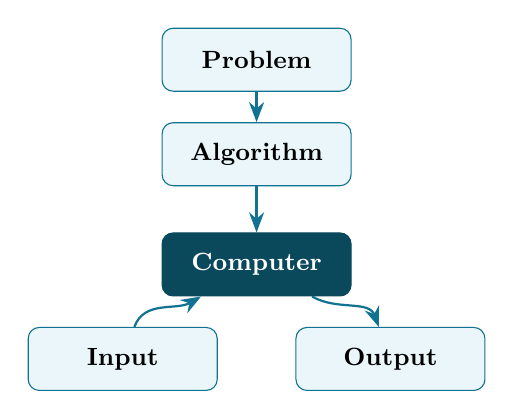
\begin{tikzpicture}[
        box/.style={draw=PrimaryMid,fill=PrimaryLight!30,rounded corners=4pt,
                    font=\small\bfseries,minimum width=2.4cm,minimum height=0.8cm,
                    text centered},
        comp/.style={draw=PrimaryDark,fill=PrimaryDark,text=white,rounded corners=4pt,
                     font=\small\bfseries,minimum width=2.4cm,minimum height=0.8cm,
                     text centered},
        arr/.style={-{Stealth[scale=1.1]},PrimaryMid,thick}
      ]
        \node[box] (prob) at (1.5,3.8) {Problem};
        \node[box] (algo) at (1.5,2.6) {Algorithm};
        \node[comp] (comp) at (1.5,1.2) {Computer};
        \node[box]  (inp)  at (-0.2,0.0) {Input};
        \node[box]  (out)  at (3.2,0.0) {Output};
        \draw[arr] (prob)--(algo);
        \draw[arr] (algo)--(comp);
        \draw[arr] (inp) to[out=70,in=210] (comp);
        \draw[arr] (comp) to[out=330,in=110] (out);
      \end{tikzpicture}
  \end{columns}
\end{frame}

\begin{frame}{Special Features of Algorithms}
  \begin{columns}[T]
    \column{0.50\textwidth}
      \begin{itemize}
        \item \keyword{Non-ambiguity} — every instruction has exactly
              one interpretation
        \item \keyword{Range of inputs} — must handle all valid inputs,
              not just examples
        \item \keyword{Multiple representations} — the same algorithm
              can be expressed as pseudocode, flowchart, or code
        \item \keyword{Multiple algorithms} — one problem can have
              many solutions
        \item \keyword{Different efficiencies} — different algorithms
              for the same problem can differ enormously in speed
      \end{itemize}
    \column{0.45\textwidth}
      \begin{exampleblock}{Same Problem, Three Algorithms}
        Computing $\gcd(60, 24)$:
        \begin{enumerate}
          \item \textbf{Euclid's algorithm} — elegant, fast
          \item \textbf{Consecutive integer checking} — slow, limited
          \item \textbf{Middle-school factoring} — complex, very slow
        \end{enumerate}
        \vspace{0.3em}
        All three give the answer \highlight{12} — but not equally fast.
      \end{exampleblock}
  \end{columns}
\end{frame}

% ============================================================
\section{Case Study — Greatest Common Divisor}
% ============================================================

\begin{frame}[shrink=12]{Problem Statement}
  \begin{block}{Greatest Common Divisor}
    Given two non-negative integers $m$ and $n$ (not both zero),
    find $\gcd(m,n)$ — the \emph{largest integer that divides both}.
  \end{block}
  \vspace{0.4em}
  \begin{columns}[T]
    \column{0.38\textwidth}
      \textbf{Examples}
      \begin{itemize}
        \item $\gcd(60,\;24) = 12$
        \item $\gcd(60,\;\phantom{0}0) = 60$
        \item $\gcd(\phantom{0}7,\;\phantom{0}5) = 1$ (coprime)
        \item $\gcd(\phantom{0}0,\;\phantom{0}0) = ?$ \alert{undefined}
      \end{itemize}
    \column{0.55\textwidth}
      \textbf{Three classical approaches}
      \vspace{0.3em}
      \scriptsize
      \begin{tabular}{lll}
        \toprule
        \textbf{Algorithm} & \textbf{Efficiency} & \textbf{Notes} \\
        \midrule
        Euclid's & \bigO{\log \min(m,n)} & Best choice \\
        Consecutive check & \bigO{n} & Fails for $n=0$ \\
        Middle-school & Very slow & Ambiguous steps \\
        \bottomrule
      \end{tabular}
  \end{columns}
\end{frame}

\begin{frame}[shrink=12]{Algorithm 1: Euclid's Algorithm}
  \begin{columns}[T]
    \column{0.50\textwidth}
      \textbf{Key insight:}
      \[
        \gcd(m,\,n) = \gcd(n,\; m \bmod n)
      \]
      Repeat until the second argument becomes 0.
      \vspace{0.5em}
      \begin{block}{Pseudocode}
        \begin{algorithmic}[1]
          \Require $m,n \geq 0$, not both zero
          \Ensure $\gcd(m,n)$
          \While{$n \neq 0$}
            \State $r \gets m \bmod n$
            \State $m \gets n$;\; $n \gets r$
          \EndWhile
          \State \Return $m$
        \end{algorithmic}
      \end{block}
    \column{0.45\textwidth}
      \textbf{Trace: $\gcd(60, 24)$}
      \vspace{0.3em}

      \begin{tabular}{>{\bfseries}c>{\bfseries}c>{\bfseries}c}
        \rowcolor{PrimaryDark}\color{white}$m$ & \color{white}$n$ &
        \color{white}$r = m \bmod n$ \\
        \rowcolor{PrimaryLight!40} 60 & 24 & 12 \\
        \rowcolor{white} 24 & 12 & \phantom{1}0 \\
        \rowcolor{PrimaryLight!40} 12 & \phantom{2}0 & — \\
      \end{tabular}
      \vspace{0.5em}

      \textbf{Result:} $\gcd(60,24) = \highlight{12}$

      \vspace{0.5em}
      \begin{alertblock}{Efficiency}
        The number of iterations is $\mathcal{O}(\log \min(m,n))$
      \end{alertblock}
  \end{columns}
\end{frame}

\begin{frame}[fragile,shrink=12]{Algorithm 1: Implementation}
  \begin{columns}[T]
    \column{0.48\textwidth}
      \textbf{Recursive version}
      \begin{lstlisting}[language=Java,numbers=none]
int gcd(int m, int n) {
    if (n == 0) return m;
    return gcd(n, m % n);
}
      \end{lstlisting}
    \column{0.48\textwidth}
      \textbf{Iterative version}
      \begin{lstlisting}[language=Java,numbers=none]
int gcd(int m, int n) {
    while (n != 0) {
        int r = m % n;
        m = n;
        n = r;
    }
    return m;
}
      \end{lstlisting}
  \end{columns}
  \vspace{0.5em}
  \begin{columns}[T]
    \column{0.50\textwidth}
      \begin{exampleblock}{Why the iterative version is preferred}
        \begin{itemize}
          \item No function-call overhead
          \item Constant stack space
          \item Same time complexity \bigO{\log n}
        \end{itemize}
      \end{exampleblock}
    \column{0.45\textwidth}
      \begin{block}{Convergence guarantee}
        After two consecutive iterations, the second argument
        decreases by \emph{at least half} — hence $\mathcal{O}(\log n)$.
      \end{block}
  \end{columns}
\end{frame}

\begin{frame}[shrink=12]{Algorithm 2: Consecutive Integer Checking}
  \begin{columns}[T]
    \column{0.50\textwidth}
      \textbf{Idea:} Start from $t = \min(m,n)$ and test each
      candidate downward until we find one that divides both.
      \vspace{0.4em}
      \begin{block}{Pseudocode}
        \begin{algorithmic}[1]
          \State $t \gets \min(m, n)$
          \While{$t > 0$}
            \If{$m \bmod t = 0$ \textbf{and} $n \bmod t = 0$}
              \State \Return $t$
            \EndIf
            \State $t \gets t - 1$
          \EndWhile
        \end{algorithmic}
      \end{block}
    \column{0.45\textwidth}
      \begin{alertblock}{Limitations}
        \begin{itemize}
          \item \important{Fails} when either input is \textbf{zero}
                ($\min(m,0)=0$, loop never runs)
          \item Worst case: $\mathcal{O}(\min(m,n))$ iterations
          \item Much slower than Euclid's for large inputs
        \end{itemize}
      \end{alertblock}
      \vspace{0.4em}
      \textbf{Example:} $\gcd(60,24)$
      \begin{itemize}
        \item $t=24$: $24 \nmid 60$ $\times$
        \item $t=23\ldots13$: $\times$ (11 wasted steps)
        \item $t=12$: $12 \mid 60$ and $12 \mid 24$ $\checkmark$
      \end{itemize}
  \end{columns}
\end{frame}

\begin{frame}[shrink=12]{Algorithm 3: Middle-School Procedure}
  \begin{columns}[T]
    \column{0.50\textwidth}
      \textbf{Steps:}
      \begin{enumerate}
        \item Find the prime factorization of $m$
        \item Find the prime factorization of $n$
        \item Identify all common prime factors (with multiplicity)
        \item Multiply them to get $\gcd(m,n)$
      \end{enumerate}
      \vspace{0.3em}
      \textbf{Example:} $\gcd(60,24)$
      \[
        60 = \textcolor{AlertRed}{2}\cdot\textcolor{AlertRed}{2}\cdot\textcolor{AlertRed}{3}\cdot 5
        \qquad
        24 = \textcolor{AlertRed}{2}\cdot\textcolor{AlertRed}{2}\cdot\textcolor{AlertRed}{3}\cdot 2
      \]
      \[
        \gcd(60,24)= \textcolor{AlertRed}{2\cdot 2\cdot 3} = \highlight{12}
      \]
    \column{0.45\textwidth}
      \begin{alertblock}{Why this algorithm is problematic}
        \begin{itemize}
          \item Prime factorization is \important{not defined
                unambiguously} in the problem — it is itself
                a hard sub-problem
          \item Step 3 ("find common factors") is also not
                clearly specified
          \item Fails when an input equals 1
          \item Overall complexity: much worse than \bigO{\log n}
        \end{itemize}
      \end{alertblock}
      \begin{exampleblock}{Lesson}
        Even a familiar school method can be a \emph{bad} algorithm.
      \end{exampleblock}
  \end{columns}
\end{frame}

\begin{frame}[shrink=12]{Sieve of Eratosthenes}
  \textbf{Goal:} Produce all primes $\leq n$ (needed by the middle-school method).
  \vspace{0.2em}
  \begin{columns}[T]
    \column{0.52\textwidth}
      \begin{block}{Pseudocode}
        \begin{algorithmic}[1]
          \For{$p \gets 2$ \textbf{to} $n$}\; $A[p] \gets p$ \EndFor
          \For{$p \gets 2$ \textbf{to} $\lfloor\sqrt{n}\rfloor$}
            \If{$A[p] \neq 0$}
              \State $j \gets p^2$
              \While{$j \leq n$}
                \State $A[j] \gets 0$;\quad $j \gets j + p$
              \EndWhile
            \EndIf
          \EndFor
          \State Output all $A[p] \neq 0$
        \end{algorithmic}
      \end{block}
    \column{0.43\textwidth}
      \textbf{Trace for $n = 25$:}
      \vspace{0.3em}

      \setlength{\tabcolsep}{3pt}
      \begin{tabular}{*{8}{c}}
        2 & 3 & \cellcolor{gray!20}\sout{4} & 5 &
        \cellcolor{gray!20}\sout{6} & 7 &
        \cellcolor{gray!20}\sout{8} & \cellcolor{gray!20}\sout{9} \\[2pt]
        \cellcolor{gray!20}\sout{10} & 11 & \cellcolor{gray!20}\sout{12} & 13 &
        \cellcolor{gray!20}\sout{14} & \cellcolor{gray!20}\sout{15} &
        \cellcolor{gray!20}\sout{16} & 17 \\[2pt]
        \cellcolor{gray!20}\sout{18} & 19 & \cellcolor{gray!20}\sout{20} &
        \cellcolor{gray!20}\sout{21} & \cellcolor{gray!20}\sout{22} & 23 &
        \cellcolor{gray!20}\sout{24} & \cellcolor{gray!20}\sout{25} \\
      \end{tabular}
      \vspace{0.4em}

      Primes $\leq 25$: \textbf{2,\,3,\,5,\,7,\,11,\,13,\,17,\,19,\,23}

      \vspace{0.4em}
      Complexity: \bigO{n \log \log n}
  \end{columns}
\end{frame}

% ============================================================
\section{Algorithm Correctness}
% ============================================================

\begin{frame}[shrink=12]{What Does "Correct" Mean?}
  \begin{block}{Definition: Correctness}
    An algorithm is \keyword{correct} if, for \emph{every} valid input,
    it terminates and produces the \emph{right output}.
  \end{block}
  \vspace{0.5em}
  \begin{columns}[T]
    \column{0.50\textwidth}
      \textbf{Why it is non-trivial:}
      \begin{itemize}
        \item The set of valid inputs is usually \emph{infinite}
        \item Testing a few examples is \important{not a proof}
        \item Intuition can be deceived by edge cases
        \item Formal proof (mathematical induction, loop invariants)
              is required
      \end{itemize}
    \column{0.45\textwidth}
      \begin{alertblock}{Common pitfall}
        "It works on the examples I tried" $\neq$ correct algorithm. \\[0.3em]
        A single \emph{counter-example} is enough to \emph{disprove}
        correctness.
      \end{alertblock}
      \begin{exampleblock}{Good practice}
        After designing an algorithm, actively try to find inputs
        where it \emph{fails}.
      \end{exampleblock}
  \end{columns}
\end{frame}

\begin{frame}[shrink=12]{Case Study: The Shortest Tour Problem}
  \begin{columns}[T]
    \column{0.55\textwidth}
      \textbf{Problem:} Given $n$ cities with known pairwise distances,
      find the \emph{shortest} round tour that visits each city exactly once
      (Travelling Salesman Problem — TSP).

      \vspace{0.5em}
      \textbf{Applications:}
      \begin{itemize}
        \item Delivery route optimization
        \item Circuit board drilling
        \item DNA sequencing
      \end{itemize}

      \vspace{0.4em}
      \textbf{Proposed heuristic: Nearest Neighbor (NN)}
      \begin{enumerate}
        \item Start at any city
        \item Repeatedly visit the \emph{nearest unvisited} city
        \item Return to the start
      \end{enumerate}
    \column{0.40\textwidth}
      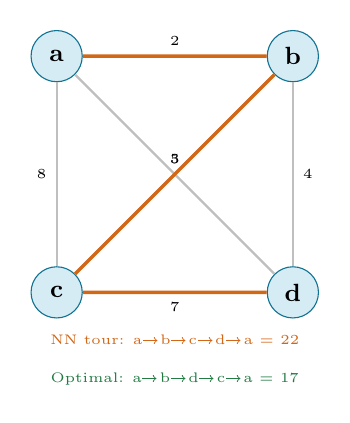
\begin{tikzpicture}[
        city/.style={circle,draw=PrimaryMid,fill=PrimaryLight!60,
                     font=\bfseries\small,minimum size=0.65cm},
        ok/.style={-{Stealth},AccentOrange,very thick},
        edge/.style={draw=gray!50,thick}
      ]
        \node[city] (a) at (0,3) {a};
        \node[city] (b) at (3,3) {b};
        \node[city] (c) at (0,0) {c};
        \node[city] (d) at (3,0) {d};
        \draw[edge] (a)--(b) node[midway,above,font=\tiny]{2};
        \draw[edge] (a)--(c) node[midway,left,font=\tiny]{8};
        \draw[edge] (a)--(d) node[midway,above,font=\tiny]{5};
        \draw[edge] (b)--(c) node[midway,above,font=\tiny]{3};
        \draw[edge] (b)--(d) node[midway,right,font=\tiny]{4};
        \draw[edge] (c)--(d) node[midway,below,font=\tiny]{7};
        \draw[ok] (a)--(b)--(c)--(d)--cycle;
        \node[font=\tiny,text=AccentOrange] at (1.5,-0.6)
          {NN tour: a→b→c→d→a = 22};
        \node[font=\tiny,text=SuccessGreen] at (1.5,-1.1)
          {Optimal: a→b→d→c→a = 17};
      \end{tikzpicture}
  \end{columns}
\end{frame}

\begin{frame}[shrink=12]{Nearest-Neighbor Counter-Example}
  \setlength{\hfuzz}{1pt}
  \raggedright\sloppy
  \begin{columns}[T]
    \column{0.55\textwidth}
      \textbf{Points on a number line:}
      \vspace{0.5em}

      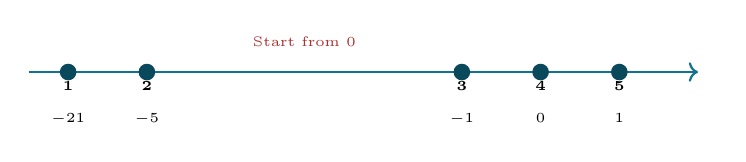
\begin{tikzpicture}
        \draw[PrimaryMid,thick,->] (-0.5,0) -- (8,0) node[right]{};
        \foreach \x/\l in {0/1,1/2,5/3,6/4,7/5}{
          \fill[PrimaryDark] (\x,0) circle(3pt);
          \node[below,font=\tiny\bfseries] at (\x,0) {\l};
        }
        \node[below=0.4cm,font=\tiny] at (0,0) {$-$21};
        \node[below=0.4cm,font=\tiny] at (1,0) {$-$5};
        \node[below=0.4cm,font=\tiny] at (5,0) {$-$1};
        \node[below=0.4cm,font=\tiny] at (6,0) {0};
        \node[below=0.4cm,font=\tiny] at (7,0) {1};
        \node[above=0.2cm,font=\tiny,text=AlertRed] at (3,0)
          {Start from 0};
      \end{tikzpicture}

      \vspace{0.5em}
      \textbf{NN from point 4 (value 0):}
      \begin{itemize}
        \item Visit 5 (dist 1), then 3 (dist 2), then 2 (dist 4),
              then 1 (dist 16), back to 4 (dist 22)
        \item Total: \important{45 units}
      \end{itemize}
      {\scriptsize\textbf{Optimal tour:} 1→2→3→4→5→1 =
      \highlight{26 units}
      }
    \column{0.40\textwidth}
      \begin{alertblock}{Conclusion}
        The Nearest-Neighbor heuristic \important{does not always}
        produce an optimal tour.
      \end{alertblock}
      \vspace{0.5em}
      \begin{block}{Key lesson}
        \begin{itemize}
          \item Seeking \emph{counter-examples} is a vital part
                of algorithm design
          \item A plausible algorithm is not necessarily a
                correct one
          \item TSP has no known efficient exact algorithm
                (it is NP-hard)
        \end{itemize}
      \end{block}
  \end{columns}
\end{frame}

% ============================================================
\section{Algorithm Efficiency}
% ============================================================

\begin{frame}{Why Efficiency Matters}
  \begin{columns}[T]
    \column{0.55\textwidth}
      \begin{itemize}
        \item Hardware improvements are \emph{incremental};
              algorithmic improvements can be \emph{exponential}
        \item A 10$\times$ faster CPU helps — switching from
              $\mathcal{O}(n^2)$ to $\mathcal{O}(n\log n)$ helps
              \emph{much more}
        \item Real systems must scale: from 10\,000 to
              10\,000\,000 users
      \end{itemize}
      \vspace{0.4em}
      \begin{alertblock}{Software always outstrips hardware}
        Even the fastest computer cannot save a poorly designed
        exponential-time algorithm for large inputs.
      \end{alertblock}
    \column{0.40\textwidth}
      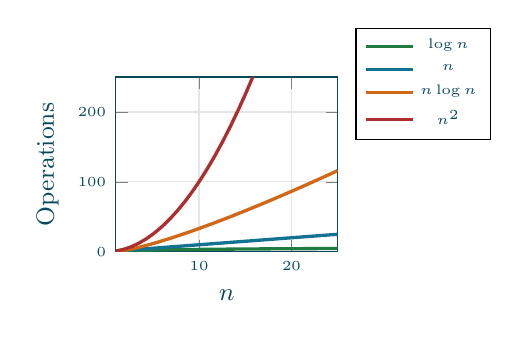
\begin{tikzpicture}
        \begin{axis}[
          width=4.4cm, height=3.8cm,
          xlabel={\small $n$},
          ylabel={\small Operations},
          xmin=1,xmax=25,ymin=0,ymax=250,
          legend style={font=\tiny,at={(1.08,0.96)},anchor=west},
          tick label style={font=\tiny},
          label style={font=\small},
          grid=major, grid style={gray!20},
          no markers,
          every axis/.style={PrimaryDark}
        ]
          \addplot[SuccessGreen,very thick,domain=1:25,samples=30]
            {ln(x)/ln(2)};
          \addplot[PrimaryMid,very thick,domain=1:25,samples=30]
            {x};
          \addplot[AccentOrange,very thick,domain=1:25,samples=30]
            {x*ln(x)/ln(2)};
          \addplot[AlertRed,very thick,domain=1:25,samples=30]
            {x*x};
          \legend{$\log n$,$n$,$n\log n$,$n^2$}
        \end{axis}
      \end{tikzpicture}
  \end{columns}
\end{frame}

\begin{frame}[shrink=12]{How to Measure Efficiency}
  \begin{columns}[T]
    \column{0.55\textwidth}
      \textbf{Machine-independent approach:}
      \begin{itemize}
        \item Analyse \emph{pseudocode}, not actual code
        \item Assume an \emph{idealized model}: each basic operation
              takes one unit of time
        \item Count the \emph{number of basic operations} as a
              function of the \emph{input size} $n$
      \end{itemize}
      \vspace{0.3em}
      \[
        T(n) \;\approx\; c_{\text{op}} \cdot C(n)
      \]
      \begin{center}
        \small
        $c_{\text{op}}$: time per operation \quad
        $C(n)$: operation count
      \end{center}
    \column{0.40\textwidth}
      \begin{block}{Typical Input Size Measures}
        \begin{tabular}{ll}
          \toprule
          \textbf{Problem} & \textbf{Size} \\
          \midrule
          Sorting & $n$ = \# elements \\
          Matrix multiply & $n\times n$ dimension \\
          Graph problems & \# vertices + edges \\
          Primality test & \# digits of $n$ \\
          \bottomrule
        \end{tabular}
      \end{block}
      \vspace{0.3em}
      \begin{block}{Typical Basic Operations}
        key comparison, addition, multiplication,
        array access
      \end{block}
  \end{columns}
\end{frame}

\begin{frame}{Faster Algorithm vs.\ Faster CPU}
  \begin{columns}[T]
    \column{0.55\textwidth}
      \textbf{Algorithm S1} (slow, on a fast machine):
      \begin{itemize}
        \item $T(n) = 2n^2$ operations, CPU @ $10^{10}$ ops/sec
        \item For $n = 10^6$: $2\times10^{12}$ ops → \alert{200 seconds}
      \end{itemize}
      \vspace{0.4em}
      \textbf{Algorithm S2} (fast, on a slow machine):
      \begin{itemize}
        \item $T(n) = 50n\log_2 n$ ops, CPU @ $10^8$ ops/sec
        \item For $n = 10^6$: $\approx 10^9$ ops → \textcolor{SuccessGreen}{\textbf{10 seconds}}
      \end{itemize}
    \column{0.40\textwidth}
      \begin{alertblock}{Takeaway}
        A \emph{better algorithm} on a \emph{slower machine} beats
        a \emph{worse algorithm} on a faster machine for large inputs.
      \end{alertblock}
      \vspace{0.3em}
      \begin{tabular}{lrr}
        \toprule
        \textbf{Algorithm} & $n=10^4$ & $n=10^6$ \\
        \midrule
        $\mathcal{O}(n^2)$       & 1.0 s   & 2.8 hr \\
        $\mathcal{O}(n\log n)$   & 0.001 s & 0.10 s \\
        $\mathcal{O}(n)$         & 0.0001s & 0.01 s \\
        \bottomrule
      \end{tabular}
      \vspace{0.2em}
      \footnotesize (Assuming $10^8$ ops/sec)
  \end{columns}
\end{frame}

% ============================================================
\section{Algorithm Design}
% ============================================================

\begin{frame}{The Algorithm Design and Analysis Process}
  \centering
  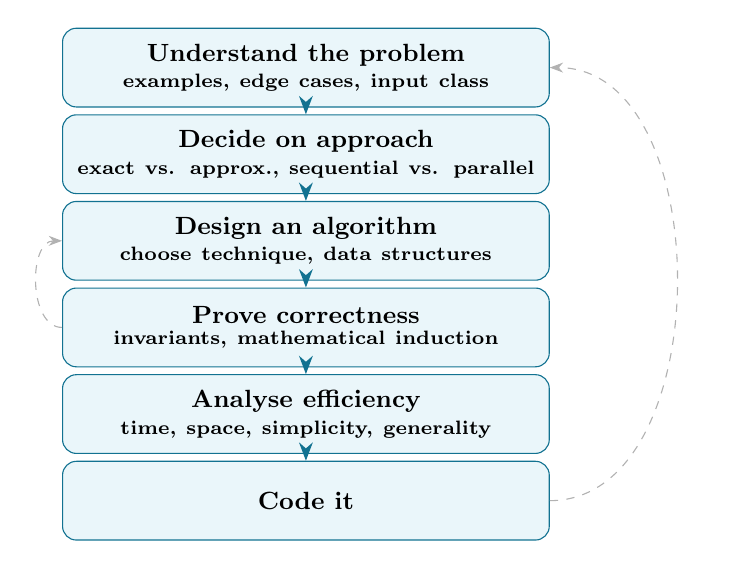
\begin{tikzpicture}[
    procbox/.style={draw=PrimaryMid,fill=PrimaryLight!30,rounded corners=5pt,
                    font=\small\bfseries,align=center,text width=5.9cm,
                    minimum height=1.0cm,inner sep=4pt},
    arr/.style={-{Stealth},PrimaryMid,thick},
    back/.style={-{Stealth},gray!60,dashed}
  ]
    \node[procbox] (understand) at (0,4.2)
      {\shortstack{Understand the problem\\\scriptsize examples, edge cases, input class}};
    \node[procbox] (decide) at (0,3.1)
      {\shortstack{Decide on approach\\\scriptsize exact vs. approx., sequential vs. parallel}};
    \node[procbox] (design) at (0,2.0)
      {\shortstack{Design an algorithm\\\scriptsize choose technique, data structures}};
    \node[procbox] (prove) at (0,0.9)
      {\shortstack{Prove correctness\\\scriptsize invariants, mathematical induction}};
    \node[procbox] (analyze) at (0,-0.2)
      {\shortstack{Analyse efficiency\\\scriptsize time, space, simplicity, generality}};
    \node[procbox] (code) at (0,-1.3) {Code it};
    \draw[arr] (understand)--(decide);
    \draw[arr] (decide)--(design);
    \draw[arr] (design)--(prove);
    \draw[arr] (prove)--(analyze);
    \draw[arr] (analyze)--(code);
    \draw[back] (prove.west) to[out=180,in=180] (design.west);
    \draw[back] (code.east)  to[out=0,in=0]   (understand.east);
  \end{tikzpicture}
\end{frame}

\begin{frame}[shrink=12]{Algorithm Design Techniques}
  \begin{columns}[T]
    \column{0.48\textwidth}
      \begin{block}{Techniques covered in this course}
        \scriptsize
        \begin{tabular}{ll}
          \keyword{Brute Force} & try all possibilities \\[3pt]
          \keyword{Decrease \& Conquer} & reduce to smaller instance \\[3pt]
          \keyword{Divide \& Conquer} & split into equal halves \\[3pt]
          \keyword{Transform \& Conquer} & change representation \\[3pt]
          \keyword{Dynamic Programming} & overlapping sub-problems \\[3pt]
          \keyword{Greedy Algorithms} & locally optimal choices \\
        \end{tabular}
      \end{block}
    \column{0.48\textwidth}
      \begin{block}{Important Problem Types}
        \scriptsize
        \begin{tabular}{ll}
          \concept{Sorting} & reorder a list \\[3pt]
          \concept{Searching} & find an element \\[3pt]
          \concept{String processing} & text, patterns \\[3pt]
          \concept{Graph problems} & paths, flows, trees \\[3pt]
          \concept{Combinatorial} & permutations, subsets \\[3pt]
          \concept{Geometric} & points, lines, hulls \\[3pt]
          \concept{Numerical} & equations, integrals \\
        \end{tabular}
      \end{block}
  \end{columns}
\end{frame}

\begin{frame}{Course Roadmap}
  \centering
  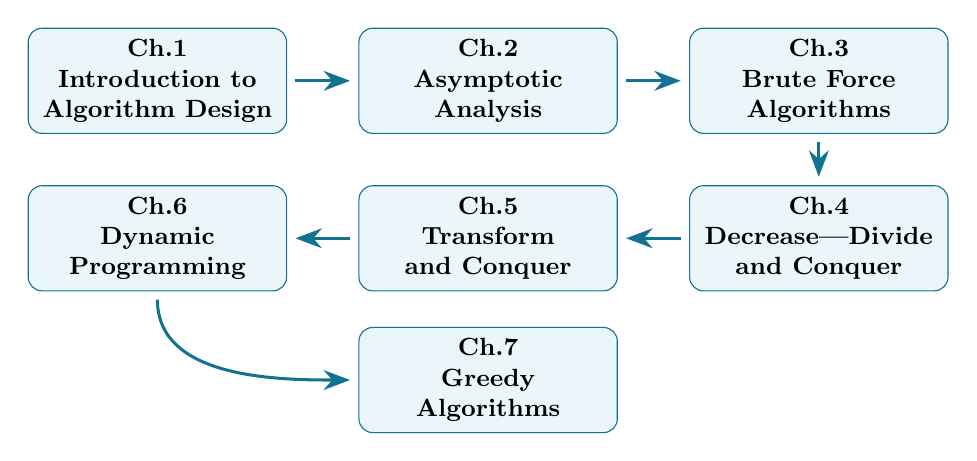
\begin{tikzpicture}[
    ch/.style={draw=PrimaryMid,fill=PrimaryLight!30,rounded corners=5pt,
               font=\small\bfseries,align=center,
               text width=3.0cm,minimum width=3.2cm,minimum height=1.1cm,
               inner sep=4pt},
    arr/.style={-{Stealth[scale=1.2]},draw=PrimaryMid,line width=1.1pt,
               shorten >=3pt,shorten <=3pt}
  ]
    \node[ch] (c1) at (0,0)     {Ch.1\\Introduction to\\Algorithm Design};
    \node[ch] (c2) at (4.2,0)   {Ch.2\\Asymptotic\\Analysis};
    \node[ch] (c3) at (8.4,0)   {Ch.3\\Brute Force\\Algorithms};
    \node[ch] (c4) at (8.4,-2.0){Ch.4\\Decrease|Divide\\and Conquer};
    \node[ch] (c5) at (4.2,-2.0){Ch.5\\Transform\\and Conquer};
    \node[ch] (c6) at (0,-2.0)  {Ch.6\\Dynamic\\Programming};
    \node[ch] (c7) at (4.2,-3.8){Ch.7\\Greedy\\Algorithms};
    \draw[arr] (c1.east)--(c2.west);
    \draw[arr] (c2.east)--(c3.west);
    \draw[arr] (c3.south)--(c4.north);
    \draw[arr] (c4.west)--(c5.east);
    \draw[arr] (c5.west)--(c6.east);
    \draw[arr] (c6.south) to[out=270,in=180] (c7.west);
  \end{tikzpicture}
\end{frame}

% ── Chapter Summary ──────────────────────────────────────────
\begin{frame}[shrink=12]{Chapter 1 Summary}
  \begin{columns}[T]
    \column{0.50\textwidth}
      \textbf{Key concepts:}
      \begin{itemize}
        \item An \keyword{algorithm} is a finite, unambiguous, effective
              sequence of steps producing a correct output
        \item The same problem can have \emph{many} algorithms with
              very different properties
        \item \keyword{Correctness} requires proof — counter-examples
              are your best diagnostic tool
        \item \keyword{Efficiency} is measured in a machine-independent
              way using asymptotic notation
      \end{itemize}
    \column{0.45\textwidth}
      \begin{exampleblock}{Three take-aways}
        \begin{enumerate}
          \item Choose algorithms — don't just code the first idea
          \item A faster algorithm on a slower machine beats a
                slower algorithm on a faster machine
        \end{enumerate}
      \end{exampleblock}
      \vspace{0.4em}
      \begin{block}{Next chapter}
        \textbf{Chapter 2:} Asymptotic analysis, Big-O, Big-$\Theta$,
        Big-$\Omega$, recurrences, and running-time calculation
      \end{block}
  \end{columns}
\end{frame}

\end{document}
